%!TEX root = report.tex

\todo[inline]{Stretchen ergens noemen}

When simulating the dynamics of cracking material, one needs a model that represents the properties of that materials, mud in our case. In \cref{ss:method:model} we present our model. \Cref{ss:method:vogel} presents the model introduced by \citeauthor{vogel2005studies2} on which ours is loosely based. So that we can contrast the two models in \cref{ss:method:contrast}.

\subsection{The model}\label{ss:method:model} \rick{Ik heb hem nagelezen. Er staat een extra todo in en ik heb de verschillende methods om veren te breken hier besproken. Zodat de implementatie sectie echt implementatie blijft.}

We use a spring simulation to model the rupture dynamics of mud. In this section we first describe the behavior and properties of one spring that connects two particles. Then we discuss a network of particles connected with springs and under which constraints this network is solved to find a stable system.

Since the cracking of mud is a very slow process we ignore Newton's and Stokes' law, i.e., we do not consider the effect of velocity and frictional forces in our model. Consequently our particles are massless and we only consider their location. This, and some other properties of our model, make it possible to find the new position of particles using a matrix vector equation, which can be solved with a linear solver.

\begin{figure}
	\centering
	  \begin{tikzpicture}
	    \node [free]  (left)  at  (0,0)   {\freeParticle{i}};
	    \node [free]  (right)   at  (4,0) {\freeParticle{j}};
	    \drawSpring{left}{right}{0}

	    \node (leftUpper) at (0,0.5) {};
	    \node (rightUpper) at (4,0.5) {};
	    \draw[dashed, <->] (leftUpper)--(rightUpper) node[foo] {$D_{ij} = \abs{x_i - x_j}$};

	    \node (leftLower) at (1,-0.5) {};
	    \node (rightLower) at (3,-0.5) {};
	    \draw[dashed, <->] (leftLower)--(rightLower) node[foo, below=1ex] {$l_0$};
	  \end{tikzpicture} %
	\caption{Illustration of a spring, \spring{0}, connecting the particles \freeParticle{i} and \freeParticle{j}. The distance between the two particles is represented by $D_{ij}$, $x_i$ and $x_j$ refer to the position of \freeParticle{i} and \freeParticle{j}, respectively. The natural length of a spring is represented by $l_0$.}
	\label{fig:method:spring}
\end{figure}

\Cref{fig:method:spring} illustrates a single connection between two particles \freeParticle{i} and \freeParticle{j}. The connection between the two particle is modeled with the spring \spring{0}. The force $F$ on a Hookean spring is defined as
%
\begin{equation}\label{eq:method:hookeslaw}
	F = -k X,	
\end{equation}
%
where $F$ is the restoring force exerted by the spring on whatever is pulling on the other end. $X$ is the displacement of the string from it's relaxed position. To ensure that the final system of equations is linearly solvable we use springs with a natural length of zero. Consequently $X$ is equal to the distance between the particles that are connected by the spring, i.e., $D_{ij}$ in \cref{fig:method:spring}. If the strain on a spring exceeds some threshold, or is among the $n$ springs with the highest strain the string breaks, and cracks appear.

In the previous paragraph we established the properties of particles and the single spring connection between them. Now we consider a network of these particles. We have opted for a uniform square grid to simulate the area of rupturing mud, see \cref{fig:model:layout}. Note that one can easily use an alternative initial layout with our model. The constants of the springs are picked from a Gaussian distribution, see \cref{s:implementation} for the details.
%
\begin{figure}
	\centering
	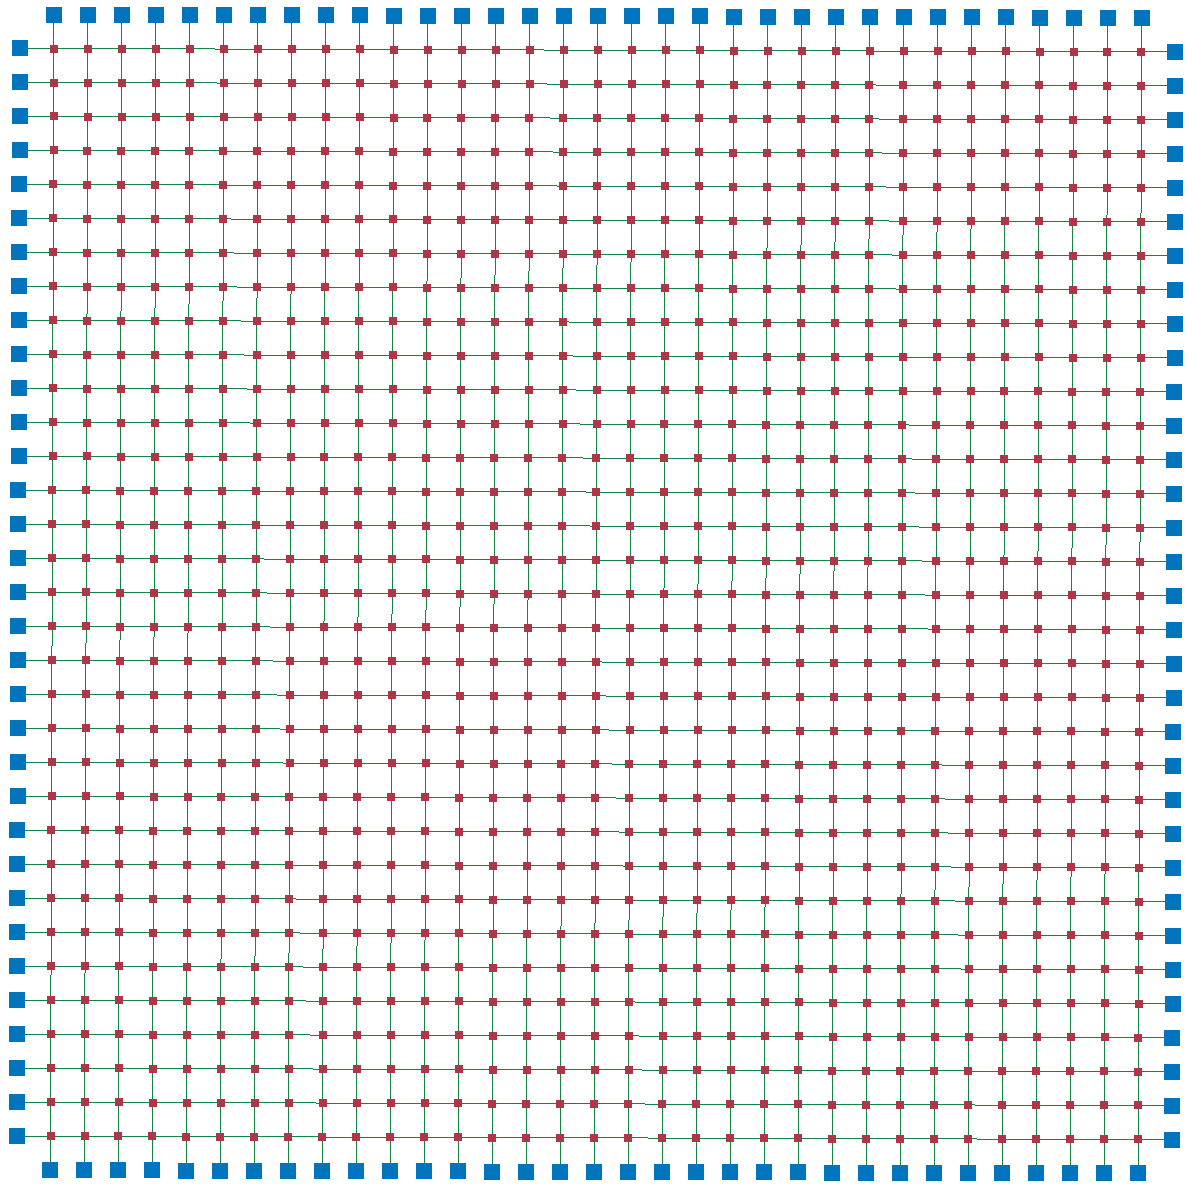
\includegraphics[width=0.9\columnwidth]{img/uniform_square_grid.png}
	\caption{Initial placement of the particles, used to represent a layer of mud without any cracks. The blue squares represent the fixed particles, whose location does not change during the simulation. The red particles change position, the green lines represent springs between the particles.}
	\label{fig:model:layout}
\end{figure}

After the grid has been initialized it needs to be stabilized. A stable state is defined as $F_i = 0 \forall_i$. Here $F_i$ is the sum of all incoming forces at a particle $v_i$, i.e.,
%
\begin{equation}\label{eq:single:force}
	F_i = - \Sigma_{j \in N_i} k_{ij} \frac{x_i - x_j}{|x_i - x_j|}[|x_i - x_j| - l_0],
\end{equation}
%
where the set $N_i$ contains the neighboring particles, and $k_{ij}$ and $l_0$ denote the spring constant and natural length of the spring connecting $v_i$ with 
particle $v_j$. The natural length of a spring is the length it would have if it is not connected to anything. To be able to use a matrix vector equation to solve, i.e., stabilize the system, we ignore the natural length by assigning a length of zero to every spring in the system. The formula from \eqref{eq:single:force} is then simplified to 
%
\begin{equation}\label{eq:single:force:simple}
	F_i = - \Sigma_{j \in N_i} k_{ij}(x_i - x_j).
\end{equation}

With the formula in \cref{eq:single:force:simple} we can now compute all the forces on every particle and move the particle to the locations, such that the system is stable, i.e., $F_i = 0 \forall_i$. With this we can find the $L$ matrix:
%
\todo[inline]{Ik dacht dat deze er hier uit zou gaan en we direct \cref{eq:method:stabilizationEquation} zouden noemen.}
\begin{equation}\label{eq:method:stabilizationEquationLHS}
	L = A^T K A .* C,
\end{equation}
%
where $A$ is the adjacency matrix, $K$ the matrix containing all the spring constants, and $C$ a correction matrix. How these matrices are constructed and what they are exactly, is discussed in \cref{s:implementation}. The system is stabilized by calculating, using the formula from \eqref{eq:single:force:simple}, the forces on all particles and moving each to the locations such that. We do this by solving the follow matrix vector equation:
%
\begin{equation}\label{eq:method:stabilizationEquation}
	L\vec{x} = \vec{r},
\end{equation}
%
where $\vec{x}$ are the unknown new particle positions. When the new locations are found, the system is stable and springs can be broken. This process of stabilizing and breaking is repeated until there are no more springs left to break. 

We propose three different methods to `break' the springs. 
%
% Break x springs with highest strain
The first methods breaks the strains with the greatest strain. The strain, $\epsilon_{ij}$,  on a spring \spring{ij} between \freeParticle{i} and \freeParticle{j} is defined as
\begin{equation}\label{eq:spring:strain}
	\varepsilon_{ij} = k_{ij} \cdot \abs{\freeParticle{i} - \freeParticle{j}},
\end{equation}
where $\spring{ij}$ represents the spring constant of the spring. If this method is used, all springs break, eventually.
%
% Break springs with strain greater than x
Alternatively one can break springs if there strain, as defined in \cref{eq:spring:strain}, is greater than some value $\varepsilon$.  If this method is used the system ends up in some stable state. This exact state is determined by the spring constants of the springs.
%
% Multiply the spring constant with some factor, instead of breaking
Instead of breaking springs, one can also consider stretching them by multiplying them with some factor $\vartheta < 0$. 

The simulation can be summarized as follows:
\begin{enumerate}[(i)]
	\item \label{it:method:init} Initialize the grid.
	\item \label{it:method:stabil} Stabilize the system, by solving \cref{eq:method:stabilizationEquation}. Consequently the particles are now shifted to their new location such that the force on every particle is zero.
	\item \label{it:method:break} Break a number of springs, e.g., the number of springs with the highest strain.
	\item \label{it:method:repeat} Repeat \cref{it:method:stabil,it:method:break} an arbitrary number of times or until the maximum number of springs has been broken.
\end{enumerate}

\subsection{The Vogel model}\label{ss:method:vogel}

The model as presented by \citeauthor{vogel2005studies2} \cite{vogel2005studies2}, differs in a number of ways. First we discuss the model and secondly the process used such that the system is stabilized and how the springs are broken. We only give a short review of the aspects of the model and simulation process to be able to give a good contrast with our model, which is presented in \cref{ss:method:model}. For detail on the model as presented by \citeauthor{vogel2005studies2} we refer the reader to \cite{vogel2005studies1} and \cite{vogel2005studies2}. 

As with our model the simple hookean springs, where the force on a spring is defined by \cref{eq:method:hookeslaw}. The network in the model of \citeauthor{vogel2005studies2} uses a triangular grid layout, where every free particle has tree neighbors. The force on a single particle is given by \cref{eq:single:force}, without the simplification of setting the natural length $l_0$ to zero. By doing this the simulation cannot be solved in one go. Including the natural length into the process makes the formula for the strain on the springs than the one used in our model, where the strain is given by \cref{eq:spring:strain}. The formula for the strain including the natural length is given by:
%
\begin{equation}\label{eq:method:strain_vogel}
	\epsilon_{ij} = \frac{|\vec{x}_i - \vec{x}_j|}{l_0} - 1.
\end{equation}

When laying out the initial grid, the spring constants are sampled from a gaussian distribution. The variance of the distribution has an effect on the material that is modeled. By choosing a high variance more heterogeneous material is modeled and consequently when a low variance is chosen the modeled material is more homogeneous.

Before springs can be broken the system of particles and springs needs to be stabilized. The breaking, and stabilization steps used by \citeauthor{vogel2005studies2} are described with the following process:
\begin{enumerate}
	\item The natural length of the springs is decreased, with an in advance chosen step size. By doing this, the strain on the springs increases, see \cref{eq:method:strain_vogel}.
	\item The springs with a strain larger than some threshold are broken.
	\item Stabilization is done radially, recursively around the broken spring. The process starts at the directly effected particles and is repeated up to a max number of steps. 
\end{enumerate}

\subsection{Contrast}\label{ss:method:contrast}

In this section we briefly review the differences between the two models that are described in \cref{ss:method:model} and \cref{ss:method:vogel}. 

\rick{Ours is fast, but does not model what it is supposed to model, but a it is a nice simulation of a breaking balloon vs Vogel who build an ultra slow but correct model of the desiccation of mud. You decide which is more fun :D. Ik had hier meer iets in gedachten dat de verschillen tussen die modellen bespreekt. Vogel heeft massless particles, maar veren hebben geen natuurlijke lengte van nul, dat soort blaat. Denk dat dat hier relevanter is. We noemen in de inleiding al waarom we dit model gebouwd hebben, anders dan het moest ;-). En in de conclusie kunnen we wel bekijken welke van de twee modellen het leukst is. Dus eignelijk de todos die hieronder staan. }

\todo[inline]{Describe the important differences of the two models.}

\todo[inline]{Story from the presentation. Different types of particles. Springs. How the particles are connected, with those springs (square uniform grid). Things like energy and what is a stable system?}

